%Content: IoT
\section{Solutions available}
In this section we will provide an overview of existing solutions which are similiar with the goal of this bachelor thesis.
\subsection{Automatic}
``The Automatic car adapter plugs into just about any car’s standard diagnostics (OBD-II) port. It unlocks the data in your car’s on-board computer and connects it to your phone via Bluetooth wireless.''\cite{automatic_how}\\
Automatic turns almost any car into a connected car. By pairing Automatic’s adapter and apps for iPhone, Android, and web, drivers are able to enhance their driving experience with a host of connected services on the Automatic platform. Automatic helps to  diagnose engine trouble, also provides acelerometer which measures car orientation to detect serious collision. By using audio signals Automatic is able to provide feedback to the driver. As Automatic connection is wireless, all data is encryptet by using 128-bit AES encryption.\cite{automatic_press} More detailed hardware specification can be found in the attachment chapter[\ref{sec:automatic_hardware_specification}]. This particular solution is proprietary and can be bought in the U.S.


\subsection{VI Monitor}
The VI Monitor  works by reading the data stream straight form vehicle electronic control unit via \gls{obd}. The VI Monitor has also  a 3.5" touch screen display and G-sensor. It has an advanced diagnostics tool with the ability to view and reset engine fault codes and comes with sophisticated comparision software. Main difference comparing Automatic and VI Monitor is in set of tools, VI Monitor allows for precision braking and acceleraion tests by using accelerometer and car data.\cite{vi_features} For more detailed overview of capabilities of VI Monitor consult [\ref{sec:vi_monitor_abilities}]


\section{Internet of Things} 
The \gls{iot} is a global infrastructure concept to further informatization of society, enabling advanced services by interconnecting things based on available technologies.\\The \gls{iot} technology aims to build a set of networks in which each object is connected. In the \gls{iot}, all objects has the storage and computing power.\cite{7263548} Through identification, data capture, communication and processing capabilities, the IoT makes full use of things to offer services to all kinds of applications. \\Whilst IoT is a hot topic in the industry it is not a new concept. It was initially put forward by Mark Weiser in the early 1990s. This concept is opening up huge opportunities for both the society and individuals. However, it also involves risks and undoubtedly represents an immense technical and social challenge.\cite{iot}
\subsection{Concept} % (fold)
\label{sub:concept}
% subsection concept (end)
``Things'', in \gls{iot} refer to a various devices. From hardware level they are all designed to do different things, collect data from various enviroments and sources. Howewer, in software aspect they behave more generally, in simplistic form it is a thing which can report data and act upon them. \\Objectification is important, because then it can be combined with many things to work together and communicate between them. Current market example could be the smart thermostat systems combining washer/dryers that use Wi-Fi for remote access.
\subsection{Benefits}
\gls{iot} is generating a lot of interest in a wide range of industries. Here are a few examples of some significant
early adopters:\\
\begin{itemize}
	\item In the healthcare field, medical device manufacturer Varian Medical Systems is seeing a 50 percent reduction
in mean time to repair their connected devices.\cite{varian_reduce} With IoT, Varian reduced customer service costs by
\$2,000 for each problem resolved remotely, with 20 percent fewer technician dispatches worldwide.
	\item Italian tire maker Pirelli is using IoT to gain valuable insights about the performance of its products in near real
time.\cite{6861917} The company is using an analytics platform to manage the huge amounts of data gathered
directly from sensors embedded in the tires in its Cyber Tyre range. The system allows the pressure,
temperature, and mileage of each tire to be monitored remotely. By keeping these factors in range, fleet
managers can have a significant impact on fuel economy and safety. In a trial covering nearly 10 million
miles, Cyber Tyres saved the equivalent of \$1,500 per truck per year\cite{5659348}.
\item Ford Motor Company’s Connected Car Dashboards program collects and analyzes data from vehicles
in order to gain insights about driving patterns and vehicle performance. The data is analyzed and
then visualized graphically using a big data platform. Among the goals are better vehicle design and
improved safety for occupants.\cite{6861917}
\item US-based HydroPoint Data Systems is using the loT in its WeatherTRAK application to enable landscape irrigation sys-tems, sensors, and computers to communicate autonomously online to identify leaks and other potential system problems. \cite{6861917}
\end{itemize}

\gls{iot} has the potential to transform the way companies make products, track goods and assets in the supply
chain, monitor the performance of systems in the field, provide security for employees and facilities,
and provide services to customers. Clearly, it’s enabling transformation in both the private and public
sectors.\newline \enquote{I firmly believe that there is not a single industry that won’t benefit from IoT.} -- said Vernon Turner, Senior Vice President of Reasearch and IoT Executive Lead at International Data Corp.(IDC). IoT is also changing the way businesses impact society and the environment. “Overall, the world needs better and more sustainable ways to live,” said Stephen Miles, research affiliate at the Center for Biomedical Innovation at the Massachusetts Institute of Technology. “To accomplish this, companies need better, more holistic models that capture a complete picture of what is happening so that they can better access
and optimize these systems.”

%Content: Big Data
% \section{Big Data}
% The rise of digital and mobile communication has made the world become more connected, networked, and traceable and has typically lead to the availability of such large scale data sets that the traditional data processing applications are insufficient. As the result new field trying to deal with this problem, have been created which scientists and computer engineers have coined `Big Data'.
% \subsection{Concept}

% \subsection{Benefits}
% \subsection{Why is it important?}
% When we will have connected car, we will need to collect information, e.g. data. With Big Data approach our solution will be scalable without need for adaptation if a very big number of devices would be connected.
\newpage
\section{I${}^2$C} % (fold)
\label{sec:i2c}
\gls{i2c} protocol is a very popular serial protocol, mainly because it is cheap, simple and allows to connect multiple devices. Whole \gls{i2c} bus can be made of only 2 lines: SDA and SCL. SDA is a data line which is carrying data from one device to another and SCL is  clock line which main purpose is to synchronize all the devices connected using the \gls{i2c} bus. The SDA and the SCL lines are mandatory for all devices which support connection using \gls{i2c} bus\cite{i2cbus}. The block diagram representation of an \gls{i2c} bus is as shown in \ref{fig:ch2}
\begin{figure}[H]
\begin{center}
\captionsetup{font=small}
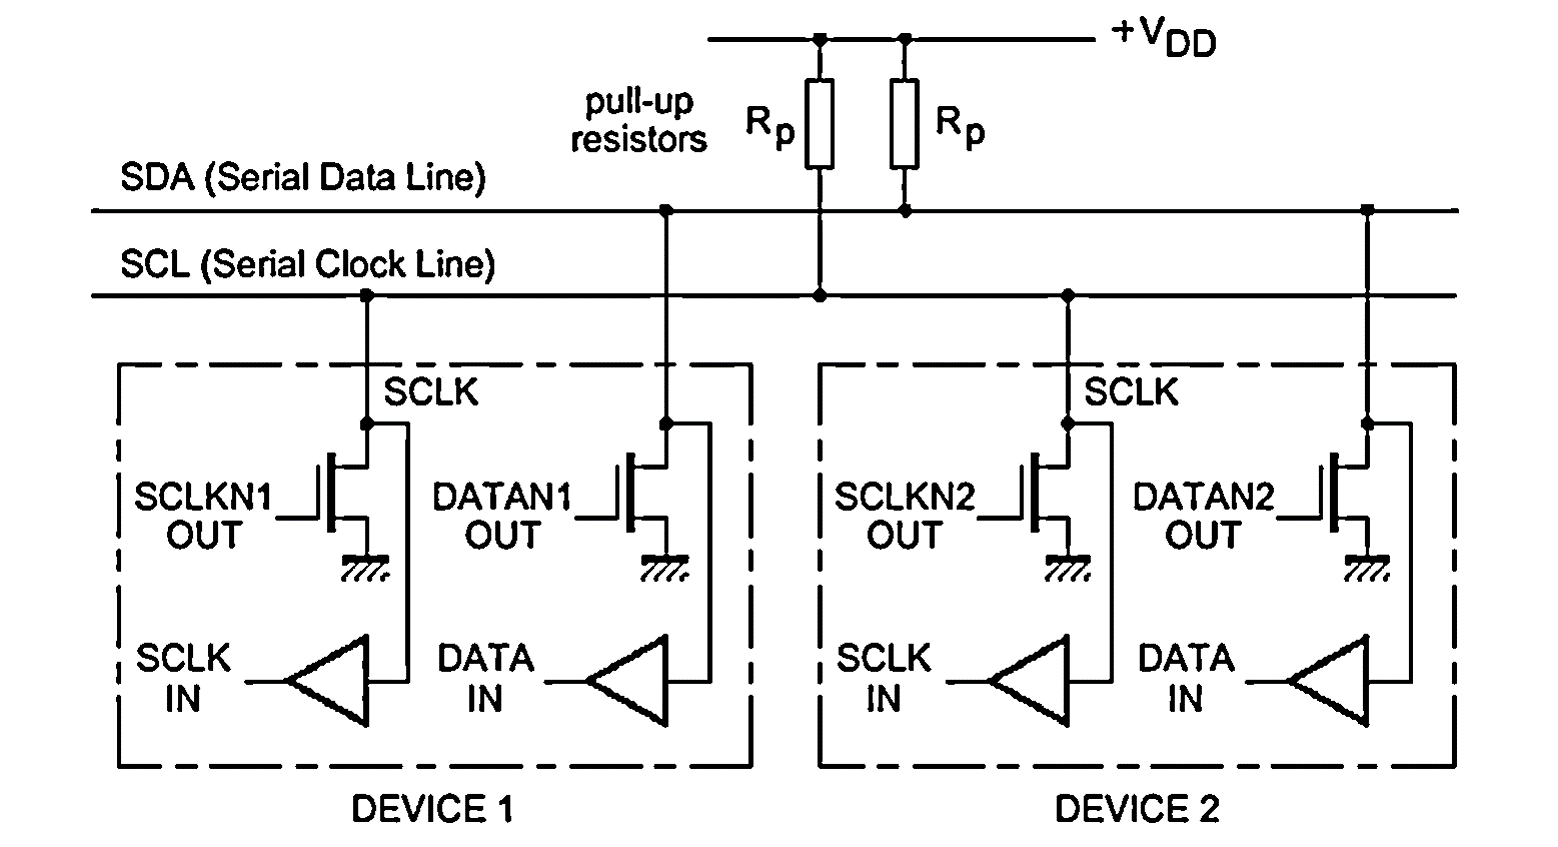
\includegraphics[scale=0.45]{pics/i2c-protocol.png}
\caption{\gls{i2c} bus.}
\label{fig:ch2}
\end{center}
\end{figure}
\subsection{Bus signals} % (fold)
 \label{sub:bus_signals}
Both signals (SCL and SDA) are bidirectional. They are connected through resistors to a positive power supply voltage. This means both lines are high when the bus is free. Activating the line means pulling it down (wired AND). The number of the devices on a single bus is almost unlimited – the only requirement is that the bus capacitance does not exceed 400 pF. Because logical 1 level depends on the supply voltage, there is no standard bus voltage.\cite{i2c_bus_signal}
 % subsection bus_signals (end)
\subsection{Hierarchy} % (fold)
\label{sub:hierarchy}
\gls{i2c} devices are can be registered as master or slave. Masters initiate a message and
slaves respond to a message. A master can have multiple slaves and any device can
be master-only, slave-only, or switch between as provided in image \ref{fig:ch1}.
\begin{figure}[H]
\begin{center}
\captionsetup{font=small}
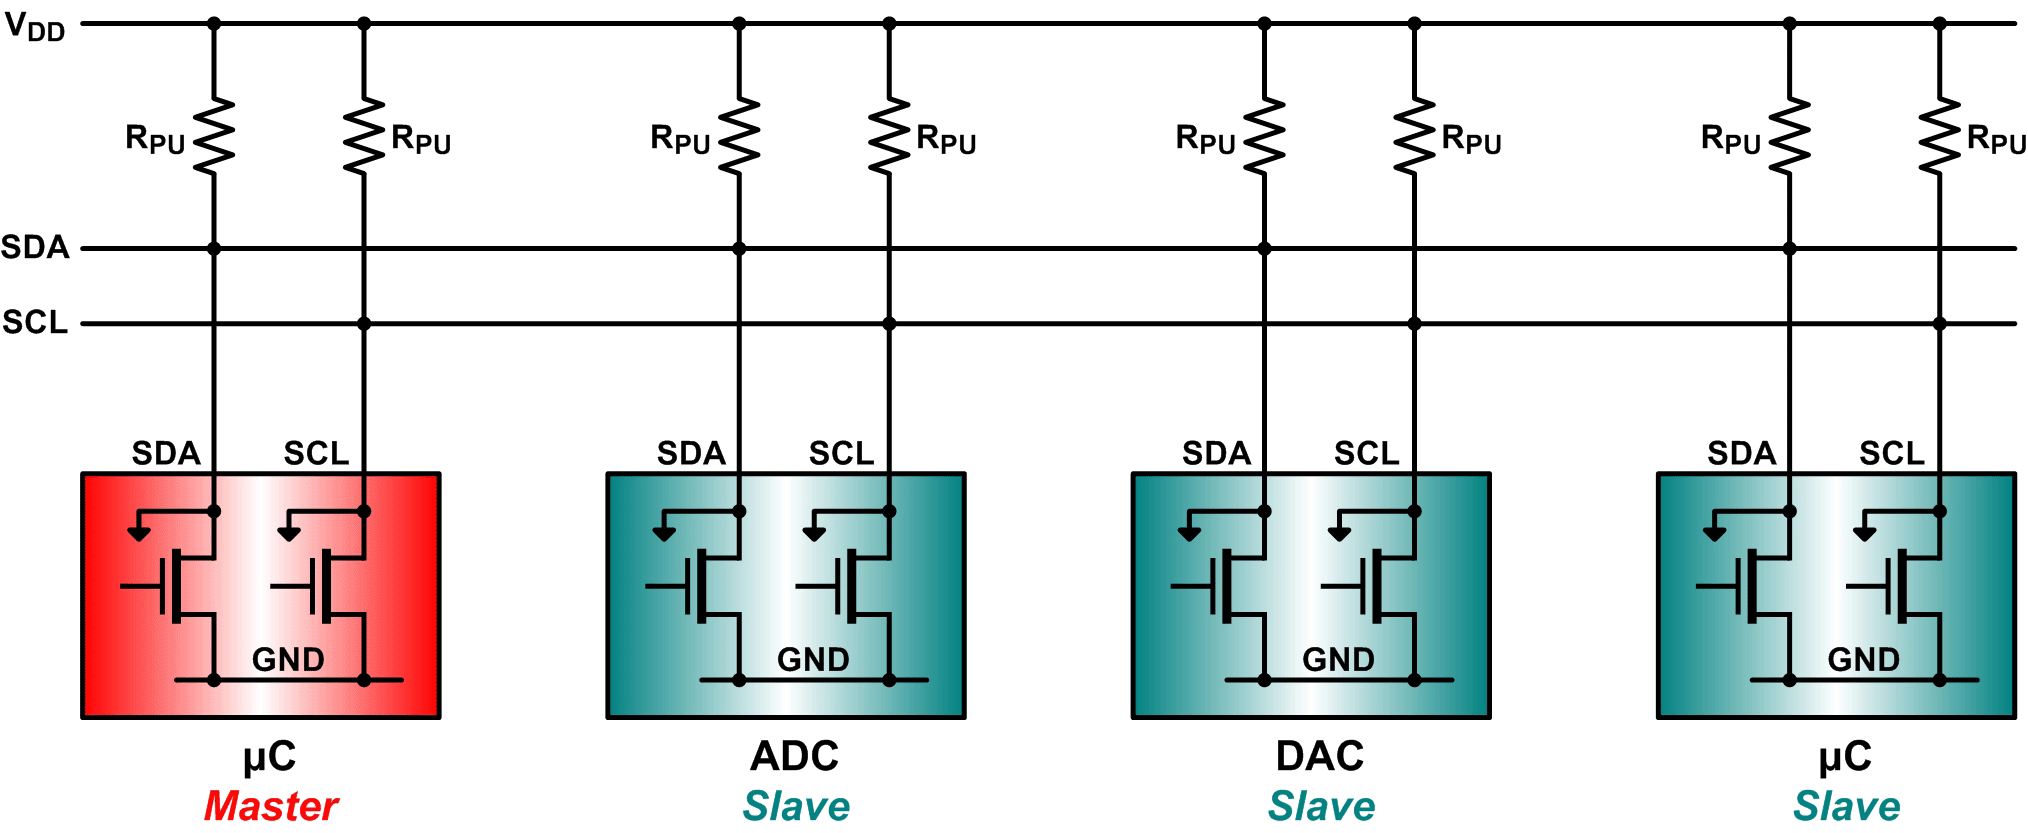
\includegraphics[scale=0.2]{pics/i2c-hierarchy.png}
\caption{Multiple \gls{i2c} devices connected on the bus.}
\label{fig:ch1}
\end{center}
\end{figure}

% section section_name (end)
\section{Single-board computer}
Sensor monitoring systems are used in many applications such as greenhouses, ecology studies, automobiles, robots, and medical devices. These systems are essentially used to study environment data like temperature, light, humidity, or air pressure. These sensor measures are used in manual and automation control based systems\cite{6028693}. The \gls{sbc} is complete functional computer built on single circuit board. It has microprocessor, memory, input/output and other features depending on the model and manufacturer. \gls{sbc} are used for educational purposes, embedded solutions and development research/systems.
\subsection{Platforms} % (fold)
\label{sub:platforms}
For making a informed decision which \gls{sbc} to use for this thesis, we provide short overview of choosen manufacturers and their platforms for embedded devices.
\subsubsection{Raspberry Pi} % (fold)
\label{ssub:raspberry_pi}
\begin{figure}[H]
\begin{center}
\captionsetup{font=small}
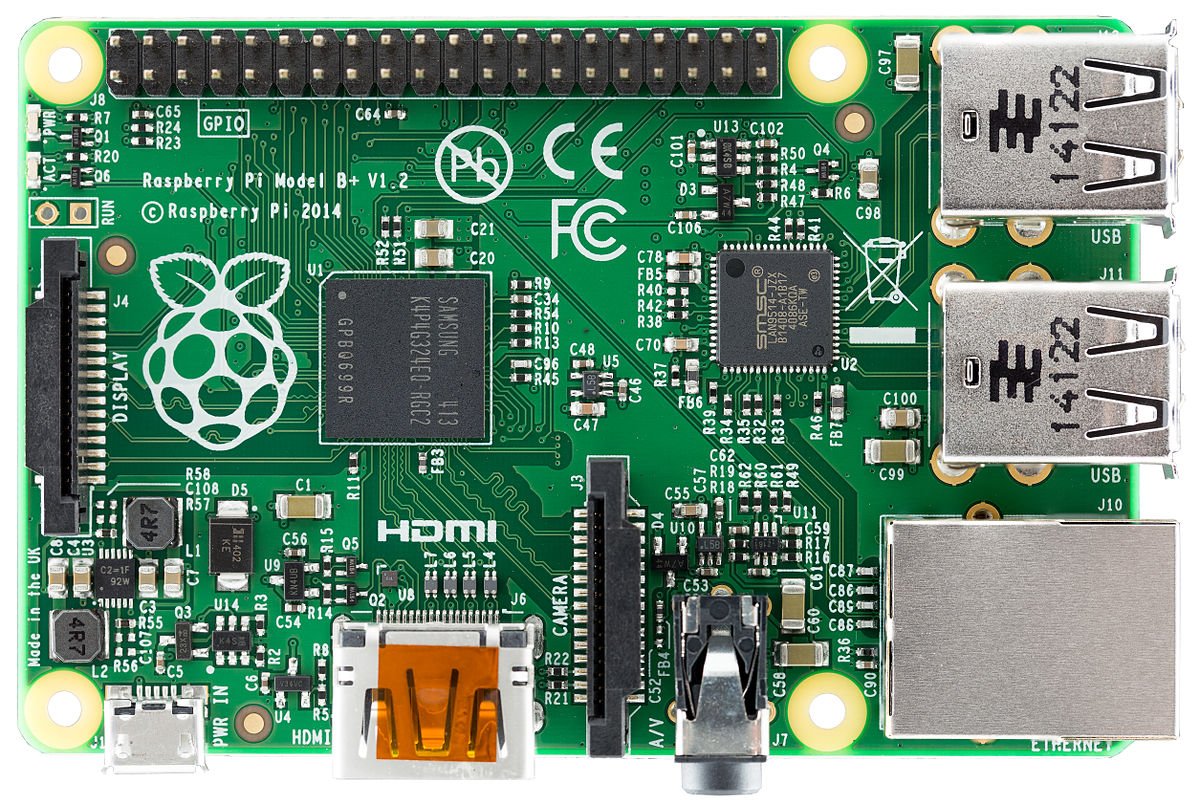
\includegraphics[scale=0.2]{pics/rasp.jpg}
\caption{Rasberry Pi Model B+ v1.2 by Lucasbosch}
\label{fig:ch3}
\end{center}
\end{figure}
Raspberry Pi is a credit-card sized mini computer as shown at Figure \ref{fig:ch3}. It is a low cost solution to many projects, and its main goal is to enable people of all ages to explore computing, and to learn how to program in languages like Scratch and Python. It is fully capable of running operating system based on ARM architecture. It has been used in a wide array of digital maker projects, from music machines and parent detectors to weather stations and tweeting birdhouses with infra-red cameras.\cite{raspberry_pi_what}. Raspberry Pi foundation develped various models with similiar hardware specifications. At the time of writing this thesis the most advanced model was Raspberry Pi 3. Hardware specifications are shown at Table \ref{tab:tab1}. Best addition to previous version was on-board wireless chip, which allowed the device to be connected to the wireless network.
\begin{table}[H]
 \begin{center}
   \begin{tabular}{l l}
   \hline
   	\textbf{SoC}: & Broadcom BCM2837\\
	\textbf{CPU}: & 4x ARM Cortex-A53, 1.2GHz\\
	\textbf{GPU}: & Broadcom VideoCore IV\\
	\textbf{RAM}: & 1GB LPDDR2 (900 MHz)\\
	\textbf{Networking}: & 10/100 Ethernet, 2.4GHz 802.11n wireless\\
	\textbf{Bluetooth}: & Bluetooth 4.1 Classic, Bluetooth Low Energy\\
	\textbf{Storage}: & microSD\\
	\textbf{GPIO}: & 40-pin header, populated\\
	\textbf{Ports}: & HDMI, 3.5mm analogue audio-video jack, 4x USB 2.0\\
	&Ethernet, Camera Serial Interface (CSI), Display Serial Interface (DSI) \\
   \hline
   \end{tabular}
 \end{center}
 \caption{Raspberry 3: Hardware specification}
 \label{tab:tab1}
\end{table}

% subsection raspberry_pi (end)
\subsubsection{The Beagles} % (fold)
\label{ssub:the_beagles}
\begin{figure}[H]
\begin{center}
\captionsetup{font=small}
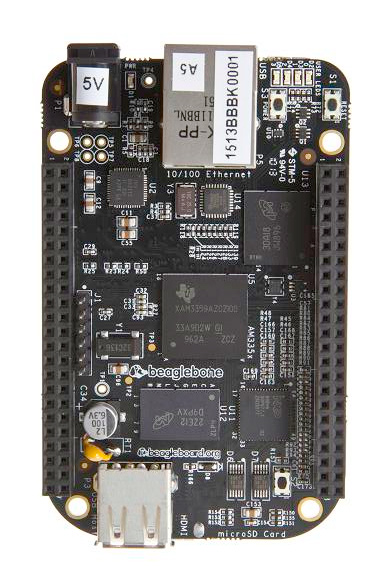
\includegraphics[scale=0.4]{pics/beagle.jpg}
\caption{BeagleBone Black}
\label{fig:ch4}
\end{center}
\end{figure}
The BeagleBoard Foundation is a US-based non-profit corporation existing to provide education in and promotion of the design and use of open-source software and hardware in embedded computing. Providing a platform for the owners and developers of open-source software and hardware to exchange ideas, knowledge and experience.\cite{beagle_what}. The Beagles are open-hardware and open-software computers, that can be used for numerous projects, same as Raspberry Pi. In time of writing this thesis most popular model among the Beagles was BeagleBone Black shown at Figure and detailed hardware specification at Table \ref{tab:tab2}.
\begin{table}[H]
 \begin{center}
   \begin{tabular}{l l}
   \hline
   	\textbf{SoC}: & Broadcom BCM2837\\
	\textbf{CPU}: & AM335x 1GHz ARM® Cortex-A8\\
	\textbf{GPU}: & SGX530 3D\\
	\textbf{RAM}: & 512MB DDR3 RAM\\
	\textbf{Memory}:& 4GB 8-bit eMMC on-board flash storage \\
	\textbf{Networking}: & 10/100 Ethernet\\
	\textbf{Storage}: & microSD\\
	\textbf{GPIO}: & 2x 46 pin headers\\
	\textbf{Ports}: & HDMI, Ethernet, LCD, GPMC,MMC1/2, 4 Serial Ports, CAN0 \\
   \hline
   \end{tabular}
 \end{center}
 \caption{BeagleBone Black: Hardware specification}
 \label{tab:tab2}
\end{table}
As we can see in comparison to Raspberry Pi, BeagleBone is a \gls{sbc} more oriented for controlling low-level application. However BeagleBone lacks any USB ports for connecting any peripherals, so to extend BeagleBone functionality one must buy expansion boars. Which is not necessarily bad, but they might not be available in common as classic USB peripherals.
% subsection the_beagles (end)
\subsubsection{The Intel® Edison} % (fold)
\label{ssub:the_intel_edison}
\begin{figure}[H]
\begin{center}
\captionsetup{font=small}
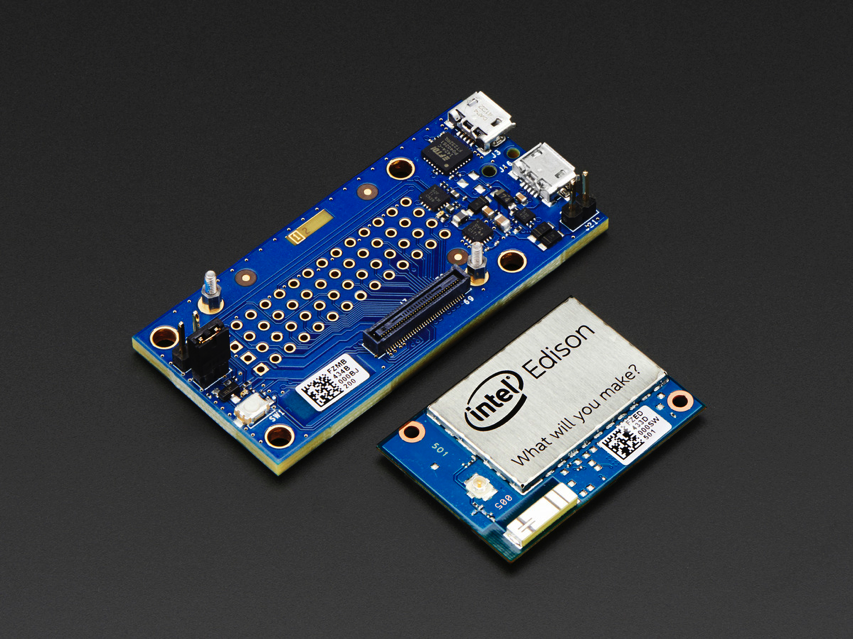
\includegraphics[scale=0.4]{pics/edison.png}
\caption{Intel® Edison with Breakout Board}
\label{fig:ch5}
\end{center}
\end{figure}
The Intel® Edison development platform is designed to lower the barriers to entry for a range of Inventors, Entrepreneurs and consumer product designers to rapidly prototype and produce IoT and wearable computing products.\cite{intel_what}\newline
Intel® Edison is very small \gls{sbc} which provides very interesting hardware specification, which can be found in Table \ref{tab:tab3}. However to connect anything to Intel® Edison, expansion board is needed because I/O pins of Intel® Edison are grouped in very small 70 PIN I/O Connector. One example of expansion board is Edison Breakout board which has a minimalistic set of features and is slightly larger than the Edison module as shown at Figure \ref{fig:ch5}. \newline This is concept which is different from the Raspberry and the Beagles. If a project needs different set of capabilities instead of changing whole \gls{sbc}, it is enough to change just the expansion board. One main disadvantage with starting with this platform is higher cost of obtaining Intel® Edison and exapnsion board.
\begin{table}[H]
 \begin{center}
   \begin{tabular}{l l}
   \hline
   	\textbf{SoC}: & 22-nm Intel® SoC\\
	\textbf{CPU}: & dual-core, dualthreaded Intel® AtomTM CPU at 500Mhz and a 32-bit \\
   	& Intel® QuarkTM microcontroller at 100 MHz\\
	\textbf{GPU}: & SGX530 3D\\
	\textbf{RAM}: & 1 GB LPDDR3 POP memory\\
	\textbf{Memory}:& 4GB eMMC\\
	\textbf{Wireless}: & Broadcom* 43340 802.11 a/b/g/n; Dual-band (2.4 and 5 GHz)\\
	& On board antenna or external antenna \\
	\textbf{Bluetooth}: & Bluetooth BT 4.0\\
	\textbf{Storage}: & microSD\\
	\textbf{GPIO}: & 70 pin headers, populated\\
	\textbf{Ports}: & USB OTG, 2 Serial Ports\\
   \hline
   \end{tabular}
 \end{center}
 \caption{Intel® Edison: Hardware specification}
 \label{tab:tab3}
\end{table}
% subsection the_intel_iot_platform (end)
% subsection platforms (end)

\subsection{Peripherals} % (fold)
\label{sub:peripherals}
To provide neccessary capabilities to solve this bachelor thesis, we might need peripheral devices to extend capabilities of developed embedded device.
\subsubsection{Bluetooth / WiFi Combination USB Dongle} % (fold)
\label{ssub:bluetooth_wifi_combination_usb_dongle}
\begin{figure}[H]
\begin{center}
\captionsetup{font=small}
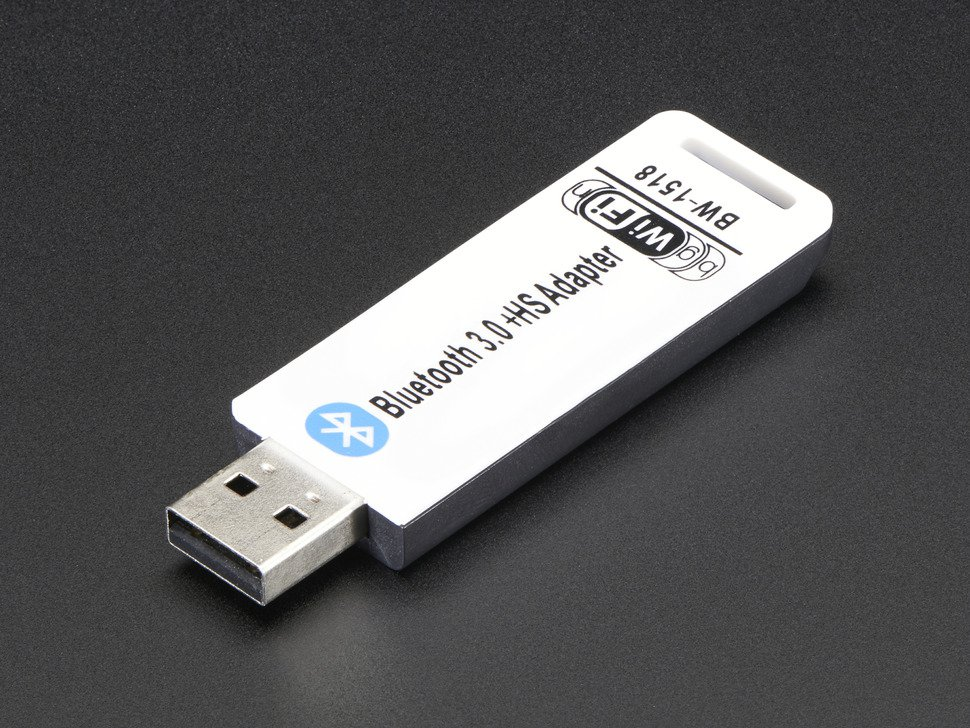
\includegraphics[scale=0.2]{pics/dongle.jpg}
\caption{Bluetooth / WiFi Combination USB Dongle}
\label{fig:wifi}
\end{center}
\end{figure}
If \gls{sbc} choosen to complete this bachelor thesis would not have WiFi/Bluetooth capabilities, this adapter in Figure \ref{fig:wifi} will be used to provide it. Technical details can be found in Chapter \ref{sec:bluetooth_wifi_combination_usb_technical_details}. Advantage of this USB dongle is that it `saves' one USB slot by integrating WiFi and Bluetooth technology into one device.
% subsubsection bluetooth_wifi_combination_usb_dongle (end)
\subsubsection{Adafruit 10-DOF} % (fold)
\label{ssub:adafruit_10_dof}
\begin{figure}[H]
\begin{center}
\captionsetup{font=small}
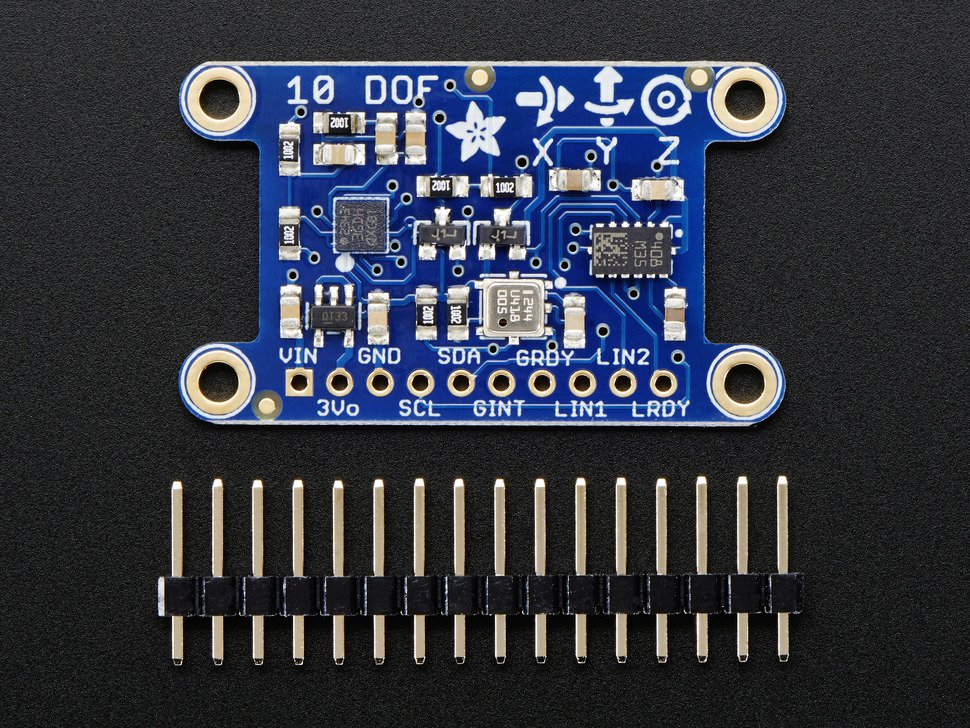
\includegraphics[scale=0.9]{pics/10dof.jpg}
\caption{Bluetooth / WiFi Combination USB Dongle}
\label{fig:10dof}
\end{center}
\end{figure}
This inertial-measurement-unit(Figure \ref{fig:10dof}) combines 3 sensors  to give you 11 axes of data: 3 axes of accelerometer data, 3 axes gyroscopic, 3 axes magnetic (compass), barometric pressure/altitude and temperature. Since all of them use I2C, you can communicate with all of them using only two wires. Most will be pretty happy with just the plain I2C interfacing, but we also break out the data ready and interrupt pins, so advanced users can interface with if they choose.\cite{ada_10dof}.
% subsubsection adafruit_10_dof (end)
\subsubsection{Adafruit FONA 3G Cellular + GPS} % (fold)
\label{ssub:adafruit_fona_3g_cellular_gps}
\begin{figure}[H]
\begin{center}
\captionsetup{font=small}
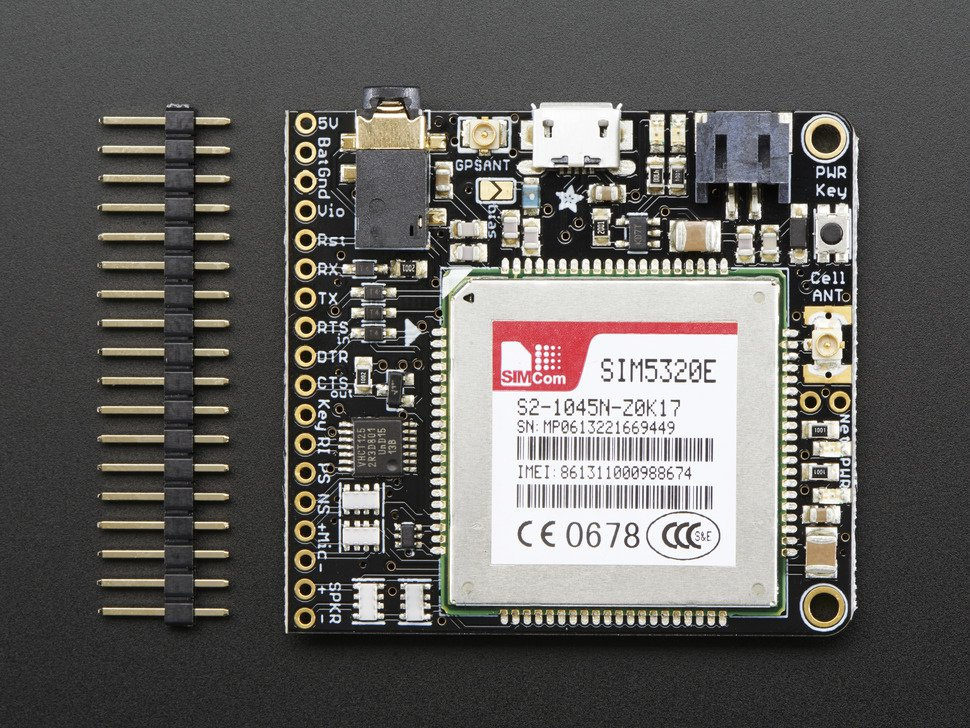
\includegraphics[scale=0.85]{pics/3g.jpg}
\caption{Adafruit FONA 3G Cellular Breakout - European version}
\label{fig:3g}
\end{center}
\end{figure}
The FONA 3G has better coverage, GSM backwards-compatibility and even sports a built-in GPS module for geolocation and asset tracking. This all-in-one cellular phone module with that lets you add location-tracking, voice, text, SMS and data to your project in a single breakout as shown in Figure \ref{fig:3g}.\cite{ada_3g}
% subsubsection adafruit_fona_3g_cellular_gps (end)
% subsection peripherals (end)


\section{Automotive electronic systems}
As we will be gathering data from electronic systems of the car, lets overview how they work, what systems and protocols are present in modern cars and how to use them to our benefit.
\subsection{Perspective} % (fold)
\label{sub:perspective}
% subsubsection perspective (end)
To gain better perspective into how complex elextronic systems in cars are, lets go back a little into history. In \citeyear{976923}, \citeauthor{976923} said in their work \citetitle{976923}:
\blockquote[\cite{976923}]{The growth of electronic systems has had implications for vehicle engineering. For example, today's high-end vehicles may have more than 4 kilometers of wiring-compared to 45 meters in vehicles manufactured in 1955. In July 1969, Apollo 11 employed a little more than 150 Kbytes of onboard memory to go to the moon and back. Just 30 years later, a family car might use 500 Kbytes to keep the CD player from skipping tracks.}
It is now 2016 and electronic systems evolved so much that you can find 100 milion lines of code in software of average modern high-end car\cite{lines_of_code}. Modern cars nowdays have more than 30-50 Electronic Control Units(\glspl{ecu}). At Figure \ref{fig:car_system} we can see network of electronic components inside a car.
\begin{figure}[H]
\begin{center}
\captionsetup{font=small}
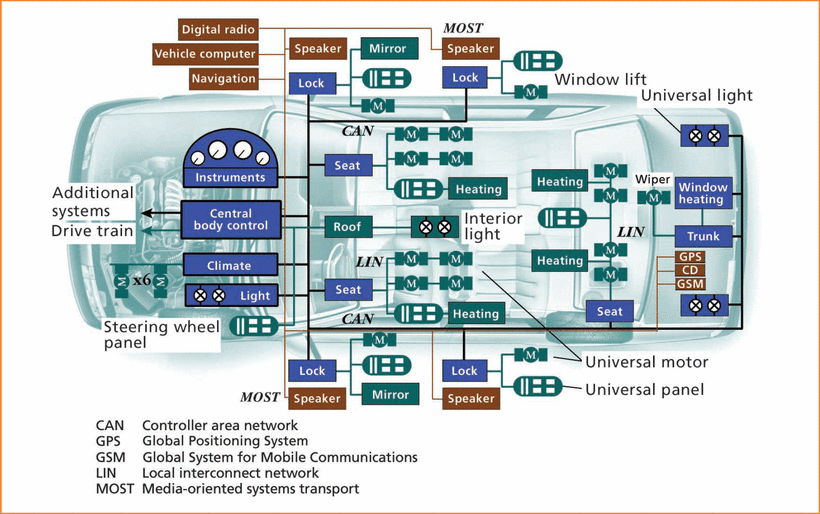
\includegraphics[scale=0.5]{pics/car_system.png}
\caption{Vehicles electronic network}
\label{fig:car_system}
\end{center}
\end{figure}
\subsubsection{In-vehicle networks} % (fold)
\label{ssub:in_vehicle_networks}
Just as \gls{lan} or Wi-Fi connects computers, control networks connects a car's electronic equipment. By interconnecting different pars of \glspl{ecu}, vehicle is able to share information amongst all distributed applications. In the history of automotive industry, wiring was just connecting element A to element B, however when electronic content in cars increased, the use of more and more cables to link elements growed enormously. To provide an example, Motorola reported in a 1998 press release, that replacing wiring cables with \gls{lan}s in the four doors of a BMW car reduced the weight by 15 kilograms. Beginning in the early 1980s, centralized and then distributed networks have replaced point-to-point wiring.\cite{815878}
% subsubsection in_vehicle_networks (end)
\subsection{Controller Area Network} % (fold)
\label{sub:controller_area_network}
The Controller Area Network(\gls{can}) is an International Standardization Organization (ISO) defined serial communications bus  specifically designed with real-time requirements in mind. Developed in the 1980s by Robert Bosch, its ease of use and low cost has led to its wide adoption throughout the automotive and automation industries\cite{788104}. It is currently the most widely used vehicular network\cite{976923}. \gls{can} is designed for signaling rates up to 1 Mbps, high protection against electrical interference, and an ability to find and repair data errors.

The \gls{can} communications protocols,  ISO 11898, conforms to the Open Systems Interconnection (OSI) model that is defined in terms of layers\cite{5116731}. Protocols specify how data travel between devices on the network. Physical layer defines how to communicate between devices which are connected. Lowest two layers of the ISO/OSI model are defined as the data-link and physical layer shown in Figure \ref{fig:iso_osi_can}.

\begin{figure}[H]
\begin{center}
\captionsetup{font=small}
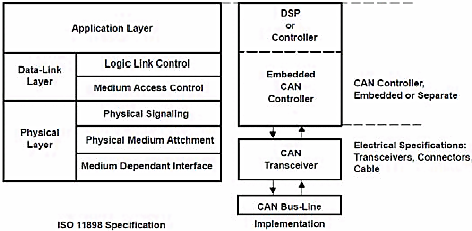
\includegraphics[scale=0.5]{pics/iso_osi_can.png}
\caption{Layers of \gls{can} Communications protocol, ISO 11898}
\label{fig:iso_osi_can}
\end{center}
\end{figure}
% subsubsection controller_area_network (end)
When data is transmitted over a \gls{can} network no individual devices are addressed. Instead, all messages have an unique identifier, a unique tag of its data content. Not only it identifies the message contents, but also the message priority as how much important data contents are. Lower the message priority, the more important message and it is delivered in prior to messages with higher priority. When a device connected to the network wants to transmit message, it passes the data and the identifier to the \gls{can} controller with a relevant request to transmit information. \gls{can} controller formats the message conents and transmits the data in form of a \gls{can} frame as shown in Figure \ref{fig:can_bus_frame}.
\begin{figure}[H]
\begin{center}
\captionsetup{font=small}
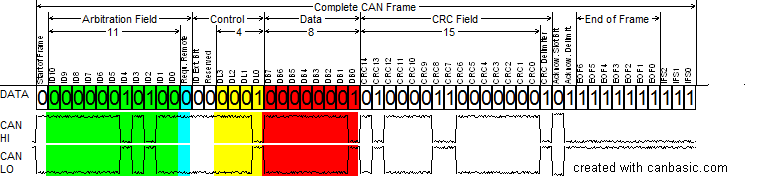
\includegraphics[scale=0.55]{pics/can_bus_frame.png}
\caption{\gls{can} bus frame, by Erniotti (output of slef programmed software) [GFDL (http://www.gnu.org/copyleft/fdl.html) or CC BY-SA 3.0 (http://creativecommons.org/licenses/by-sa/3.0)], via Wikimedia Commons}
\label{fig:can_bus_frame}
\end{center}
\end{figure}
\subsection{Conclusion} % (fold)
\label{sub:conclusion}
By understanding standard messaging protocol used in cars, we are able to read and create messages. Creating and reading messages relies on correct construction of data payload and assignment of correct identifier to the message, however specification of how to create this particular parts of the message is not publicly available, moreover specification is proprietary and probably different for every car manafacturer. To discover what data in messages are and what identifier are used, data analysis of closed data dumps from different states of the car(Ignition on, windows down, engine off, etc.) can be used, however this method is dependant on concrete make and model of the car, and is not suitable for large scale applications or general use.
% subsection conclusion (end)
\section{OBD-II}
When environmental pollution became a world issue in the 1970s, the U.S. created the Environmental Protection Agency (\gls{epa}). \gls{epa} established a new standard to limit the environmental pollutants emitted from vehicles. The car makers devised an electronic control system for the fuel supply and ignition devices, based on the standard. In addition, the Society of Automotive Engineers (\gls{sae}) established OBD in 1988 as a standard for the plug connector and on-board diagnosis system\cite{IJCSNS} as shown in Figure \ref{fig:obd_pinout}.
\begin{figure}[H]
\begin{center}
\captionsetup{font=small}
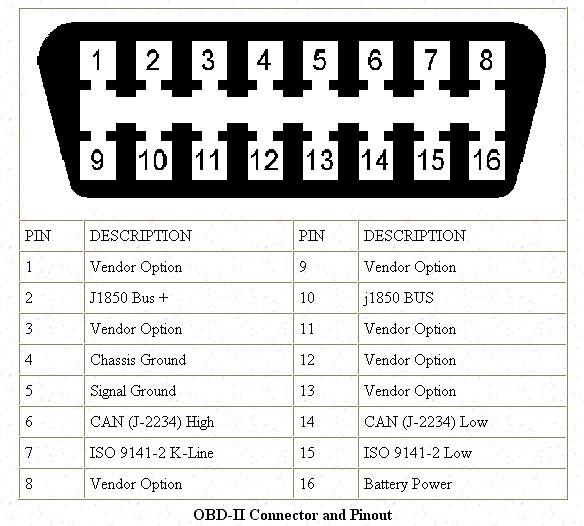
\includegraphics[scale=0.5]{pics/obd_pinout.jpg}
\caption{Pinout of the plug connector}
\label{fig:obd_pinout}
\end{center}
\end{figure}
OBD standard developed over-time and in time of writing this thesis OBD-II is standard which is used in the industry.
\subsection{Standard}
The \gls{obd} standard specifies the type of the connector and its pinout, the messaging format and electrical signalling protocols available. Difficulties may arise because of the deficiency in the OEM specific implementation of the standard. According to The OBD Home Page: There are five basic OBD protocols in use, each with minor variations on the communication pattern between the on-board diagnostic computer and the scanner console or tool. Formula CAN is the newest protocol added to the OBD specification, and it is mandated for all 2008 and newer model years\cite{7223296}. \gls{oem} provides a list of vehicle queries which can be send to the \gls{obd} port for diagnostics and gathering real-time parameters, but the list may vary from car to car. Each of this queries has a specified response on how to decode returned data again by \gls{oem} and may vary from another manufacturer respones. Finally, the OBD-II standard provides an extensible list of DTCs(Diagnostic trouble codes). As a result of this standardization, a single device can query the on-board computer(s) in any vehicle \cite{obdiso}, however this is again based solely on \gls{oem} so for getting all posible informations from the \gls{obd} port, specifiaction from \gls{oem} is needed.
\subsection{Communication}
As mention above to access information from sensors attached to a vehicle via a \gls{obd} port, special codes called Parameter IDs(\gls{pids}) are used. Typically a process of retrieving data from vehicle trough \gls{obd} port is as follows.
\begin{figure}[H]
\begin{center}
\begin{enumerate}
	\item Requested PID is entered either through connected computer or scan tool.
	\item Request is send to vehicle \gls{can} bus.
	\item Device which is responsible for given PID recognizes it and then reports the value back to the bus
	\item Connected computer or scan tool reads the response.
\end{enumerate}
\captionsetup{font=small}
\label{fig:bul1}
\caption{Query \gls{obd} process}
\end{center}
\end{figure}
From Figure 1.13 we can see that  \gls{obd} port is in simple terms subset of \gls{can} frames. Identifier and data payload is supplemented from \gls{obd} protocol based on concrete PID query.
\subsection{Conlusion} % (fold)
\label{sub:conlusion}
Main advantage of \gls{obd} port is that obtaing a single parameter from the car is relatively simple. It is enough to know correct PID to query to send, but it is not suitable for real-time telemetry, because of repetiton rate of the available data. The more different data is read out, the lower repetition time will be for each queried type, due to the fact that information is only accessible by question answer basis.
% subsection conlusion (end)
% \section{Accelerometer}
% An accelerometer measures proper acceleration which is the acceleration it experiences relative to freefall, and is the acceleration that is felt by people and objects. Put another way, at any point in spacetime the equivalence principle guarantees the existence of a local inertial frame, and an accelerometer measures the acceleration relative to that frame.\cite{einstein_rel}As a consequence an accelerometer at rest relative to the Earth's surface will indicate approximately 1 g upwards, because any point on the earth's surface is accelerating upwards relative to a local inertial frame. To obtain the acceleration due to motion with respect to the earth, this "gravity offset" should be subtracted.\\
% The reason for the appearance of a gravitational offset is Einstein's equivalence principle\cite{equivalence}, which states that the effects of gravity on an object are indistinguishable from acceleration of the reference frame. When held fixed in a gravitational field by, for example, applying a ground reaction force or an equivalent upward thrust, the reference frame for an accelerometer (its own casing) accelerates upwards with respect to a free-falling reference frame. The effect of this reference frame acceleration is indistinguishable from any other acceleration experienced by the instrument.
% An accelerometer will read zero during free fall. This includes use in a spaceship orbiting earth, but not a (non-free) fall with air resistance where drag forces reduce the acceleration until terminal velocity is reached, at which point the device would once again indicate 1 g acceleration upwards.\\
% For accident detection we will use accelerometer to determine if accident occured\cite{accident}. 
\section{Node.js} % (fold)
\label{sec:node_js}
Node.js is a event-based network application which allows developers to use asynchonous programming interfaces for I/O operations. Language which is primarily used with Node.js platform is JavaScript. Despite it is one of the newer platforms available, Node.js has significant communicty of developers and we can see more and more applications build in the industry on top of the Node.js. Node.js is built on a V8 JavaScript Engine.
\subsection{V8 JavaScript Engine} % (fold)
\label{sub:v8_javascript_engine}
\glsdesc{v8} is an open source enginge developed by Google for the Chrome web browser. \gls{v8} is open source high-performance JavaScript engine, written in C++. V8 implements ECMAScript as specified in ECMA-262, 5th edition, and runs on Windows (XP or newer), Mac OS X (10.5 or newer), and Linux systems that use IA-32, x64, or ARM processors. In several benchmark tests, V8 is many times faster than JScript (in Internet Explorer), SpiderMonkey (in Firefox), and JavaScriptCore (in Safari).\cite{google_v8}
% subsection v8_javascript_engine (end)
\subsection{Event Loop Mechanism} % (fold)
\label{sub:event_loop_mechanism}
Every Node.js application runs a single-threaded continuous event loop, which sources out time-consuming tasks to worker threads, which callback the main event loop when tasks is finised, as shown in Figure \ref{fig:node_js_model}.
\begin{figure}[H]
\begin{center}
\captionsetup{font=small}
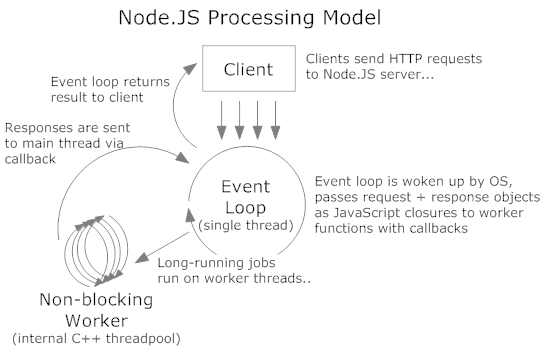
\includegraphics[scale=0.8]{pics/node_js_model.png}
\caption{Node.js Process Model}
\label{fig:node_js_model}
\end{center}
\end{figure}
Event-driven programming offers more scalable alternative than multithreaded programming, that provide developers with much more controll over application behavior and activities. In this model, the application firstly registers interest of certain events, such as disconnection of the client, data ready to be read, end of stream, etc. Then application waits to be notified of occurence in these registered events, and can act upon triggering. \cite{7073454} When an event happens a record of the event is added to the Node.js event queue, after main thread  looks at the event queue and takes the first event from the front and starts running the corresponding event handler. After event handler finishes the thread controll goes back to the main thread which again looks at the event queue if there are any events left to process.\cite{5617064}
\subsection{Asynchronous Model} % (fold)
\label{sub:asynchronous_code}
\subsubsection{Problem} % (fold)
\label{ssub:problem}
% subsubsection problem (end)
Now we know that single threaded event system works by placing events in a queue and process them one after another by calling appropriate event handler. The event handler then runs until all applications registered for that event are completed and returns control to the dispatcher, which looks again at the event queue for another event. This is an asynchronous system because order of execution of application code is not guaranteed. The order is based on event triggering which can not be pre-determined. To put it another way, order of the application written by event-driven model might be any of the combination of events which that concrete application react to. However, problem might be of the single threading, as Node.js is.\\
The reason is simple, what if event handler takes too much time to finish, or the worst case scenario never returns thread control to the dispatcher  -- application seems to freeze. Event handler never ends, so no other event handler from event queue ever gets to run.
\subsubsection{Solution} % (fold)
\label{ssub:solution}
Solution is simply use event handler to set up new thread and get it to do all the work. Ater that event handler returns at one and the new thread can process time consuming work. Problems of synchronization arise when creating a new thread in single-threaded application. In Node.js time-consuming functions are dispatched to non-blocking workers as shown in Figure \ref{fig:node_js_model}. Synchonization problem is we do not know when worker finishes with particular function, and usually we would like to process return value of that function somewhere else in the code. This problem might be solved in many ways, but all of them are nearly variations on the idea of passing an explicit someting to do when function has finished - i.e callbacks. Callback is function which will be executed at the end of function dispatchet to the worker, which successfuly solves problem of how and when to process return value of unknown time running function.\cite{asynch}
% subsubsection solution (end)
% subsection asynchronous_i_o (end)
% subsection event_loop_mechanism (end)
% section node_js (end)




